\section{Data Analysis: Community}
\label{sec:community}

The greenhouse gas emissions from a given \event is in direct proportion to
the average distance traveled by the participants of this \event.
To understand emissions, we must therefore estimate the nature of the
communities that attend each conference.

The aggregated information we describe below falls into two main categories:
first, the demographic distribution of the participants to the conferences
conditioned by various factors, and second, the participation habits of the
community through recurring participation to a given conference and the
overlap in participation between different conferences.

%% Through this section, we present the results of our data analysis in a
%% neutral way. We point out phenomena that came out as a
%% surprise to us, but defer opinionated observations and practical conclusions to
%% Section~\ref{sec:opinions}.

\subsection{Demographics: Where Did Participants Come From?}
\label{subsec:demo}

\begin{figure}
  \centering
  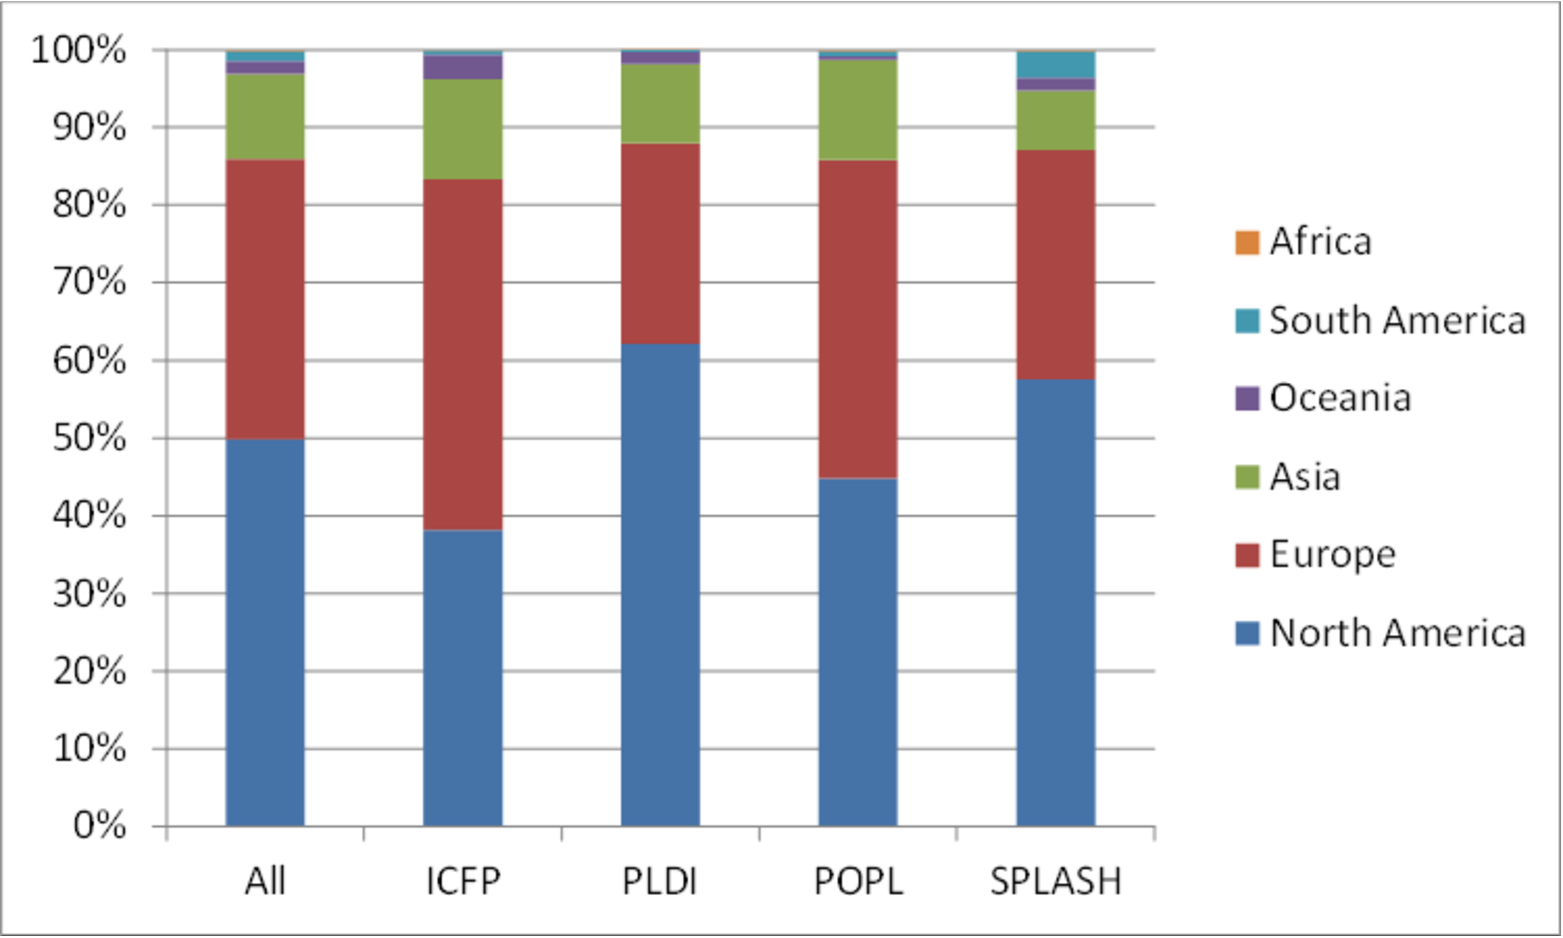
\includegraphics[width=0.7\textwidth]{ParticipantsOrigin.pdf}
  \caption{Overall origin of participants per conference.}
  \label{fig:demo-per-conf}
\end{figure}

\begin{table}
    \centering
    \csvreader[%
      head to column names,
      tabular={|c|c|c|c|c|c|c||c|},
      table head=\hline \bfseries Conference & \bfseries EU (\%) & \bfseries NA (\%) & \bfseries AS (\%) & \bfseries SA (\%) & \bfseries AF (\%) & \bfseries OC (\%) & \bfseries Local (\%)\\\hline,
      table foot = \hline,
      late after line=\ifthenelse{\equal{\Conference}{Any}}{\\\hline}{\\},
    ]{../../output/sigplan/demographic_per_conf.csv}{}{%
      \Conference & \EU & \NA & \AS & \SA & \AF & \OC & \Local \
    }

   \caption{For each kind of conference, distribution of participants per continent of origin.
     Among all participants of a category of conferences, displays the percentage of these participants that traveled from the indicated continent. The \textbf{Local} column uses for each instance of the conference the same continent as the one the conference took place in. The line \emph{Any} computes the same data, but across all conferences at once.
   }
\label{table:demo-per-conf}
\end{table}


Figure~\ref{fig:demo-per-conf}\footnote{The graphical representations in
  this preliminary draft are based on a slightly different version of our
  dataset than the one used by our tool. There may be some minor
  discrepancies between these representations and the raw tables
  presented.\bcp{Hopefully we can remove this!  Or, if it's just the big
    red-and-green table, we can at least move this comment there.}} and Table~\ref{table:demo-per-conf} show
where all participants came from, grouped by ``continents'': North and South
America, Europe, Asia, Africa, and Oceania. For each conference, we depict the
distribution of attendance per continent. Table~\ref{table:demo-per-conf}
shows the portion of attendants originating from the same continent as the
one the event took place in. To a first approximation, maximizing this last
metric, i.e. hosting conferences in the continent containing the majority of
its community, is a good thing.

Taken as a whole, these conferences attracted 50\% of their participants
from North
America, 36\% from Europe, 11\% from Asia, 2\% from Oceania, 1\% from South
America, and less than 0.2\% from Africa.
The data also shows some degree of geographical affinity for the
various conferences:
PLDI and SPLASH appear to be quite North-America-centric, while
ICFP's core community has a strong anchor in Europe as well.

\begin{table}
  \centering
  \csvreader[%
    head to column names,
    tabular={|c|c||c|c|c|c|c|c||c|},
    table head=\hline \bfseries Event & \bfseries Location & \bfseries EU (\%) & \bfseries NA (\%) & \bfseries AS (\%) & \bfseries SA (\%) & \bfseries AF (\%) & \bfseries OC (\%) & \bfseries Local (\%)\\\hline,
    table foot = \hline,
    late after line=\\,
  ]{../../output/sigplan/demographic.csv}{}{%
    \Conference~\Year & \Continent & \EU & \NA & \AS & \SA & \AF & \OC & \Local \
  }
  \caption{For each \event, the continent in which it took place and
    the distribution of attendance per continent of origin of participants.
    The final column indicates the
    portion of participants that did not change continent to attend the conference.}
  \label{table:demo-per-event}
\end{table}

\begin{figure}
  \centering
  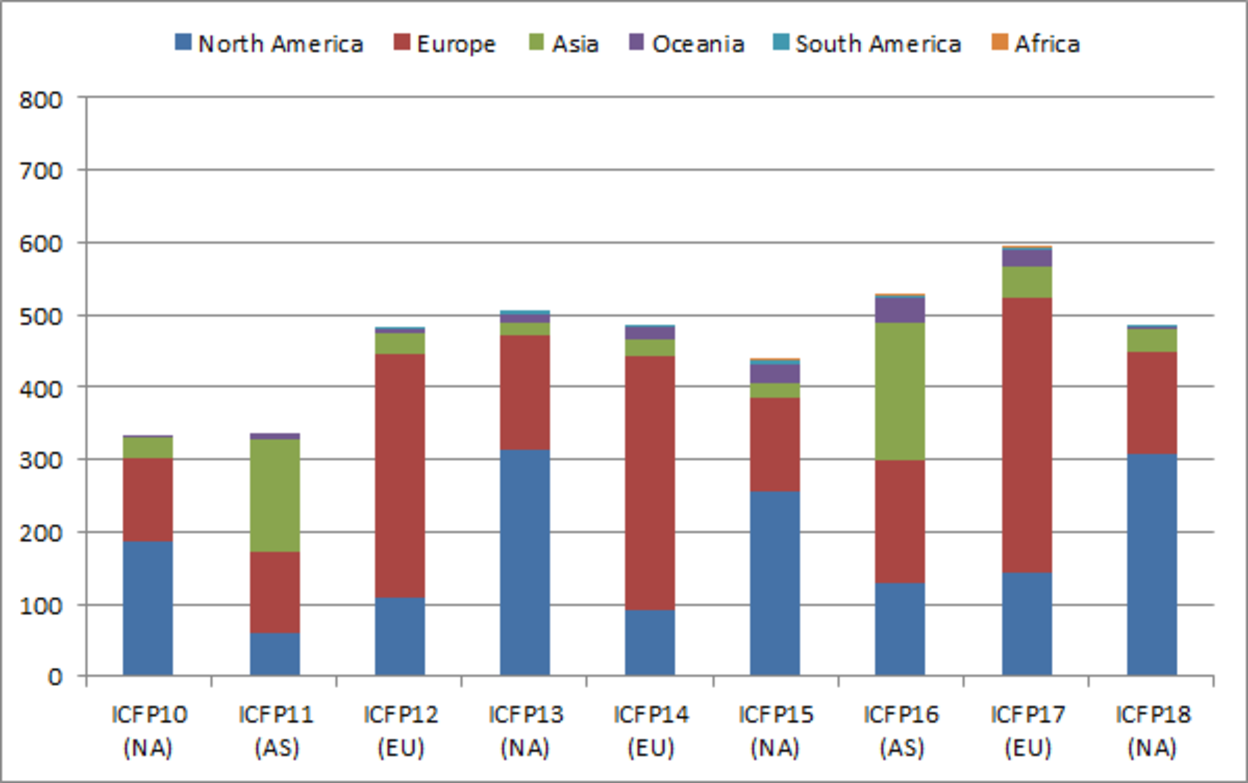
\includegraphics[width=0.45\textwidth,height=1.8in]{ParticipantsOriginICFP.pdf}
  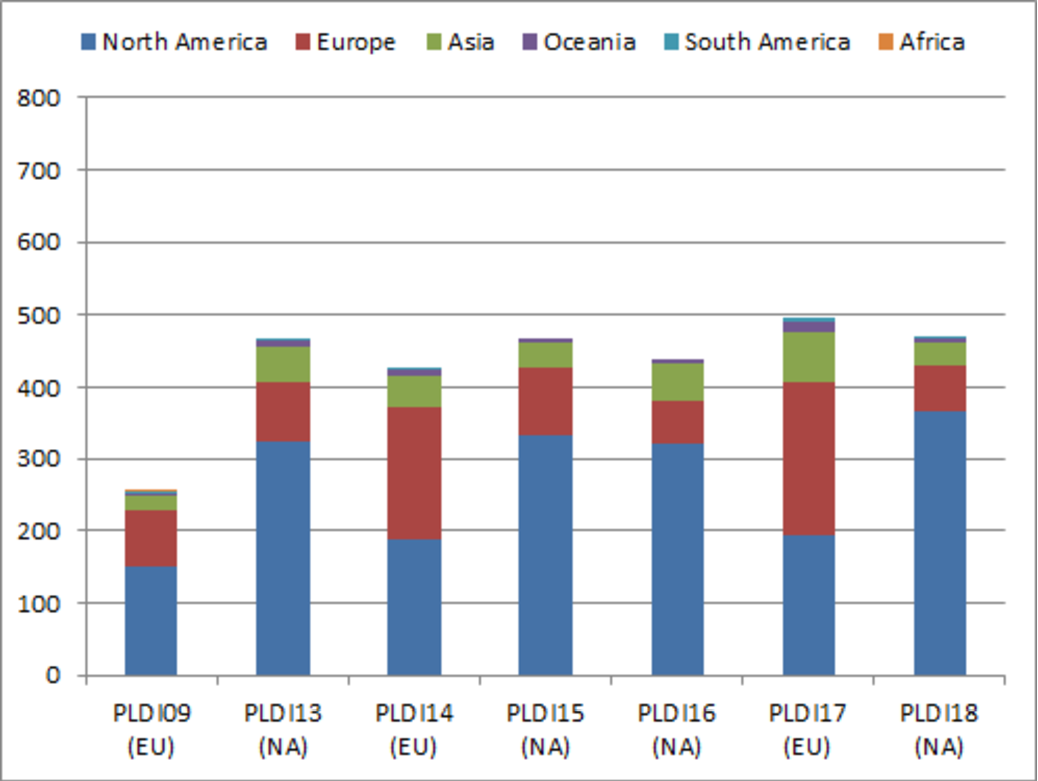
\includegraphics[width=0.45\textwidth,height=1.8in]{ParticipantsOriginPLDI.pdf}
  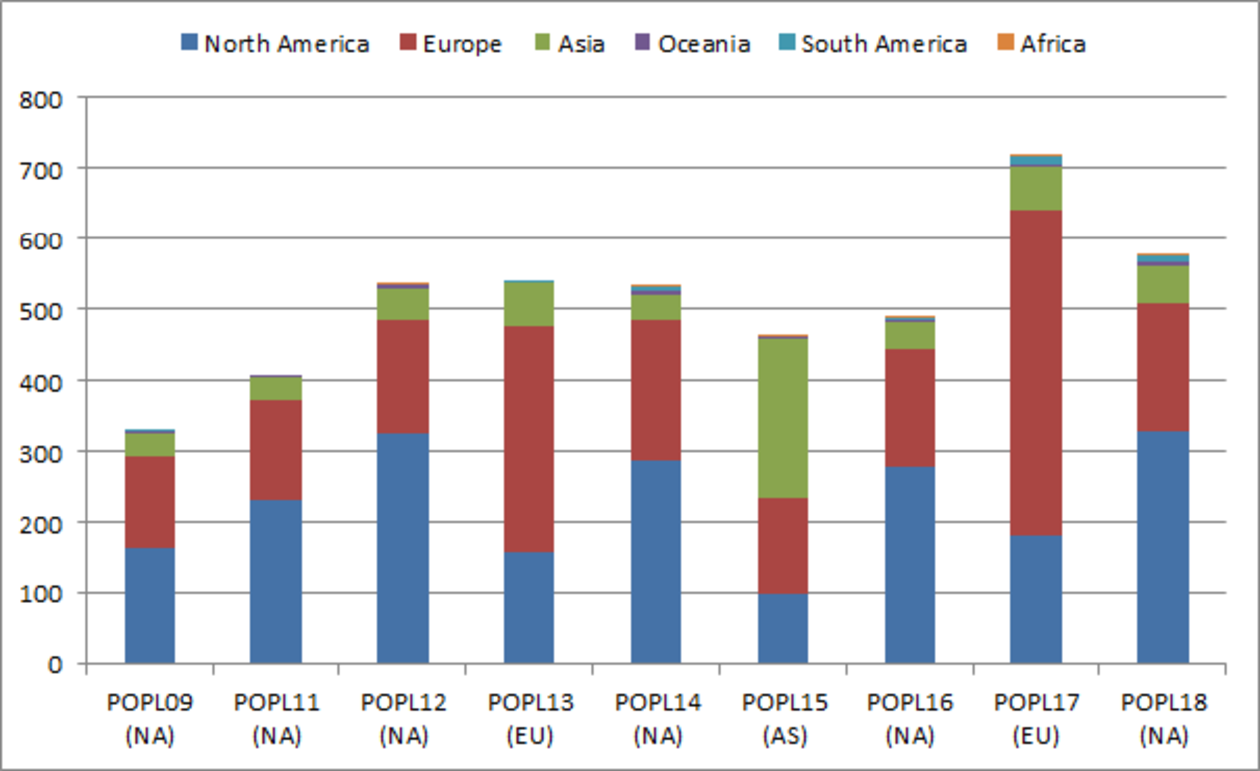
\includegraphics[width=0.45\textwidth,height=1.8in]{ParticipantsOriginPOPL.pdf}
  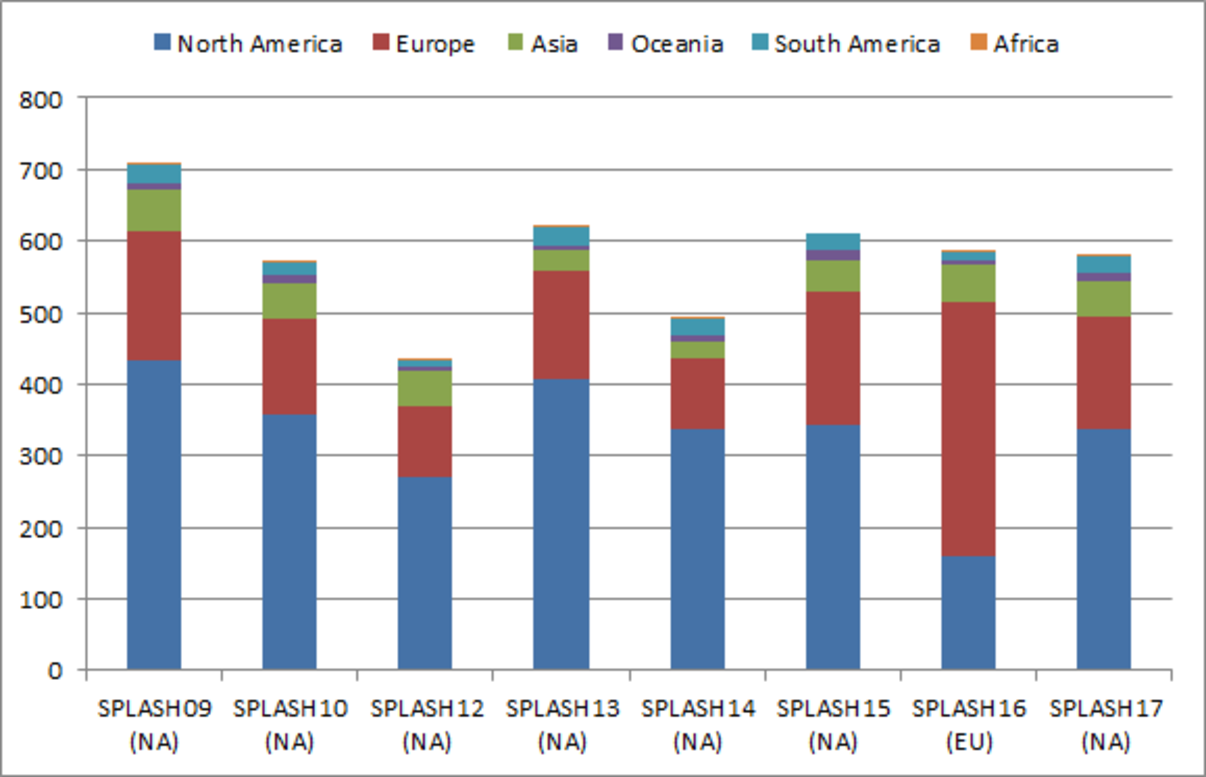
\includegraphics[width=0.45\textwidth,height=1.8in]{ParticipantsOriginSPLASH.pdf}
  \caption{Origin of participants for each conference, detail.}
  \label{fig:demo-per-event}
\end{figure}

This overall picture, however, hides some interesting facts pertaining to the
relationship between the conferences' locations and the origin of the participants.
Indeed, aggregating the attendance per conference intrinsically rests upon the
assumption of a uniform community that attends every instance of the conference
every year.  This picture turns out to be quite misleading.

Table~\ref{table:demo-per-event} and Figure~\ref{fig:demo-per-event}
show a more detailed breakdown of the origin of participants for each
conference, showing also the geographic region where the conferences were held.
%
These charts make it clear that the location of the conference had a
substantial effect on the distribution of attendees, with each conference
tending to attract people from the same geographic area. This
effect is quite visible for ICFP and POPL, with noticeable ups and downs of
the colored bars between North American and European participants when the
conferences were located in North America and Europe, respectively. Most
strikingly, Asian participation during POPL '15, ICFP '11 and ICFP '16,
events that took place on the Asian continent, is significantly higher than
the rest: there appears to be a strong locality phenomenon
here. Cross-referencing this data
with Table~\ref{table:footprint}, one can also notice that the only time
SPLASH took place in Europe also turned out to be the least carbon-intensive
edition, challenging the previous observation, based on a high-level view
of past attendance data, that the conference might appear to
be mostly North-America-centric.

\begin{table}
  \centering
  \csvreader[%
    head to column names,
    tabular={|c||c|c|c|c|c|c||c|},
    table head=\hline \bfseries Location & \bfseries EU (\%) & \bfseries NA (\%) & \bfseries AS (\%) & \bfseries SA (\%) & \bfseries AF (\%) & \bfseries OC (\%) & \bfseries Local (\%)\\\hline,
    table foot = \hline,
    late after line=\ifthenelse{\equal{\Location}{Any}}{\\\hline}{\\},
  ]{../../output/sigplan/demographic_delta.csv}{}{%
     \Location & \EU & \NA & \AS & \SA & \AF & \OC & \Local 
  }
  \caption{Geographical distribution of participation conditioned by the
    location of the \event: each row indicates the continent in which the
    conference took place, and each cell of this row depicts the percentage of
    participants of these conferences that originated from a given continent.
    The column \textbf{Local} corresponds to the same continent as the conference.}
\label{table:local_effect}
\end{table}

Table~\ref{table:local_effect} attempts to measure this locality effect. The
table depicts, all conferences being considered at once, the geographical
distribution of attendance conditioned by the geographical location of the
\event. The Asian phenomenon previously hinted at is here extremely
apparent: while overall, on average, 10.9\% of the participants come from Asia,
this number is roughly multiplied by a factor 4 when the \event takes place
in Asia (without any significant drop in total volume of attendance that
could indirectly bump this percentage).
Interestingly, this phenomenon also exists in the case of Europe (+22.29\%
deviation from the average) and North America (+12.15\% deviation from the
average).
Thus, despite their name, individual instances of international conferences
appear to exhibit a fairly strong local component.

Overall, this data shows that the goal of increasing geographic inclusion was,
indeed, accomplished by organizing the conferences in diverse parts
of the world. It also places Figure~\ref{fig:demo-per-event} in a broader
context:
a naive interpretation of that chart might lead us to conclude that North
America and Europe are where most of this community is, but it is not that
simple. Because of the regional effect on participation, the distribution of
participants also reflects the fact that most of these conferences were {\em
  held} in
North America and Europe (30), only a few were held in Asia (3), and none in
South America, Oceania, or Africa.

The situation may be summed up in two elementary observations:
\begin{obs}
  The vast majority of participants are split between North America and
  Europe, with the remainder mostly coming from
  Asia. SPLASH and PLDI are strongly anchored in North
  America. ICFP and POPL fairly equally split between North America and Europe.
  \label{obs:dist-naive}
\end{obs}
This distribution, however, is \emph{strongly} dependent on the
location of the \event.
\begin{obs}
  There is also a strong locality effect in conference attendance: nearby
  conferences attract significant numbers of new participants from the area,
  while longer distances discourage some participants.
  \label{obs:locality}
\end{obs}

\subsection{How Often Did Participants Attend These Conferences?}
\label{subsec:overlap}

Section~\ref{subsec:demo}, through the study of the demographic distribution of
attendance, has suggested the existence of local communities that only
partake in conferences when they take place close to their place of residency.
One can conversely look for groups of ``regular attendees'' that participate in
a given \conf regardless of where it is held.

\begin{figure}
  \centering
  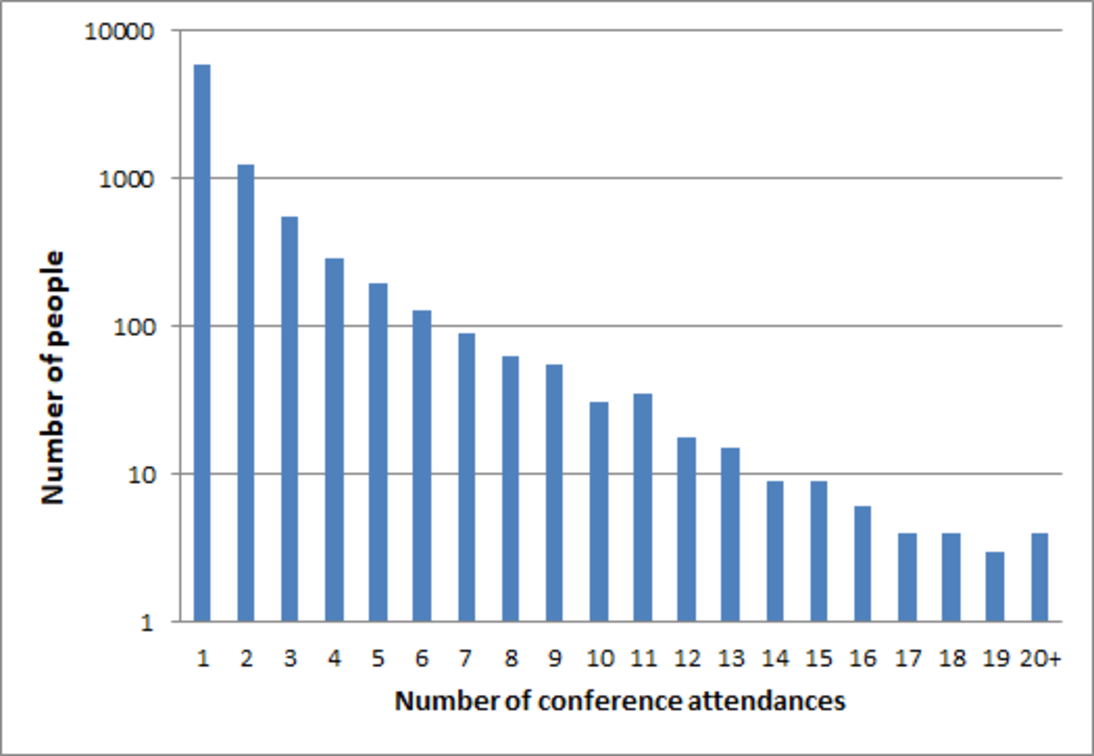
\includegraphics[width=0.6\textwidth]{AttendanceHist.pdf}
  \caption{Histogram of attendance.}
  \label{fig:hist_attendance}
\end{figure}

\begin{figure}
  \centering
  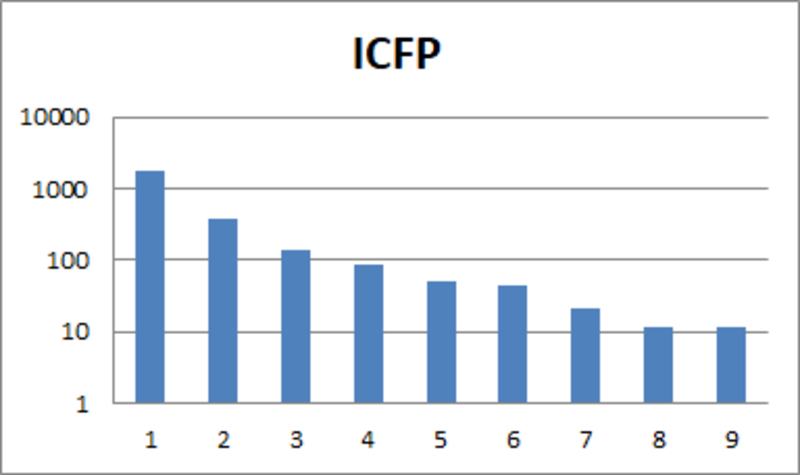
\includegraphics[width=0.45\textwidth,height=1.5in]{AttendanceHistICFP.pdf}
  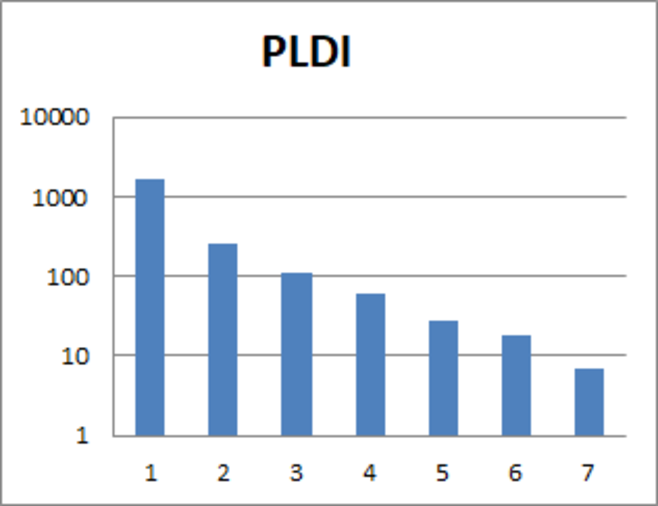
\includegraphics[width=0.4\textwidth,height=1.5in]{AttendanceHistPLDI.pdf}
  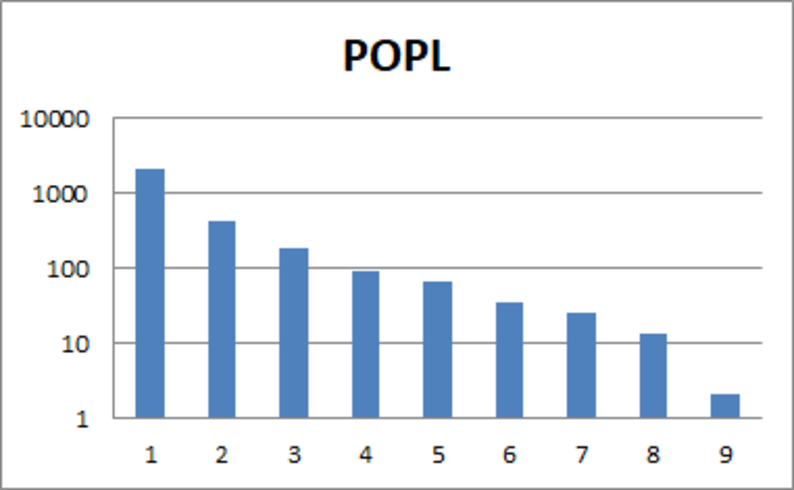
\includegraphics[width=0.45\textwidth,height=1.5in]{AttendanceHistPOPL.pdf}
  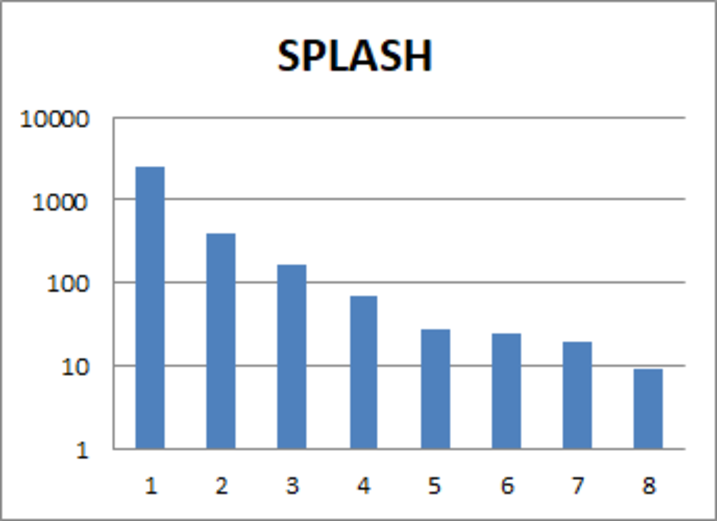
\includegraphics[width=0.4\textwidth,height=1.5in]{AttendanceHistSPLASH.pdf}
  \caption{Histogram of attendance for each conference series.}
  \label{fig:hist_attendance_per_conference}
\end{figure}

Figure~\ref{fig:hist_attendance} shows how often the same participants attended
multiple conferences. At the extremes, 6,009 people (69\%) attended only 1
conference, and just 4 people attended 20 or more conferences. Participation is
dominated by single-conference participants, perhaps reflecting a large and
transient student population. The pattern is similar for each conference series,
shown in Figure~\ref{fig:hist_attendance_per_conference}.


\subsection{What Was the Participation Overlap Between These Conferences?}

We now take a closer look at the habits of these recurring participants.

\begin{table}
  \centering
  \begin{subtable}[!t]{0.48\textwidth}
    \centering
    \csvreader[%
      head to column names,
      tabular={|c|c|c|c|},
      table head=\hline \bfseries Year & \bfseries Overlap & \bfseries \#ICFP & \bfseries \#POPL \\\hline,
      table foot = \hline,
      late after line=\ifthenelse{\equal{\Year}{All}}{\\\hline}{\\},
    ]{../../output/sigplan/overlap_cross_conf_ICFP_POPL.csv}{}{%
      \Year & \Overlap & \csvcoliii & \csvcoliv
    }
    \caption{ICFP and POPL}
  \end{subtable}
  \hspace{\fill}
  \begin{subtable}[!t]{0.48\textwidth}
    \centering
    %% \flushright
    \csvreader[%
      head to column names,
      tabular={|c|c|c|c|},
      table head=\hline \bfseries Year & \bfseries Overlap & \bfseries \#POPL & \bfseries \#PLDI \\\hline,
      table foot = \hline,
      late after line=\ifthenelse{\equal{\Year}{All}}{\\\hline}{\\},
    ]{../../output/sigplan/overlap_cross_conf_POPL_PLDI.csv}{}{%
      \Year & \Overlap & \csvcoliii & \csvcoliv
    }
    \caption{POPL and PLDI}
  \end{subtable}
  \newline
  \vspace*{0.1cm}
  \newline

  \begin{subtable}[!t]{0.48\textwidth}
    \centering
    \csvreader[%
      head to column names,
      tabular={|c|c|c|c|},
      table head=\hline \bfseries Year & \bfseries Overlap & \bfseries \#POPL & \bfseries \#SPLASH \\\hline,
      table foot = \hline,
      late after line=\ifthenelse{\equal{\Year}{All}}{\\\hline}{\\},
    ]{../../output/sigplan/overlap_cross_conf_POPL_SPLASH.csv}{}{%
      \Year & \Overlap & \csvcoliii & \csvcoliv
    } 
    \caption{POPL and SPLASH}
  \end{subtable}
  \hspace{\fill}
  \begin{subtable}[!t]{0.48\textwidth}
    \centering
    %% \flushright
    \csvreader[%
      head to column names,
      tabular={|c|c|c|c|},
      table head=\hline \bfseries Year & \bfseries Overlap & \bfseries \#ICFP & \bfseries \#PLDI \\\hline,
      table foot = \hline,
      late after line=\ifthenelse{\equal{\Year}{All}}{\\\hline}{\\},
    ]{../../output/sigplan/overlap_cross_conf_ICFP_PLDI.csv}{}{%
      \Year & \Overlap & \csvcoliii & \csvcoliv
    }
    \caption{ICFP and PLDI}
  \end{subtable}
  \newline
  \vspace*{0.1cm}
  \newline

  \begin{subtable}[!t]{0.48\textwidth}
    \centering
    \csvreader[%
      head to column names,
      tabular={|c|c|c|c|},
      table head=\hline \bfseries Year & \bfseries Overlap & \bfseries \#ICFP & \bfseries \#SPLASH \\\hline,
      table foot = \hline,
      late after line=\ifthenelse{\equal{\Year}{All}}{\\\hline}{\\},
    ]{../../output/sigplan/overlap_cross_conf_ICFP_SPLASH.csv}{}{%
      \Year & \Overlap & \csvcoliii & \csvcoliv
    }
    \caption{ICFP and SPLASH}
  \end{subtable}
  \hspace{\fill}
  \begin{subtable}[!t]{0.48\textwidth}
    %% \flushright
    \centering
    \csvreader[%
      head to column names,
      tabular={|c|c|c|c|},
      table head=\hline \bfseries Year & \bfseries Overlap & \bfseries \#PLDI & \bfseries \#SPLASH \\\hline,
      table foot = \hline,
      late after line=\ifthenelse{\equal{\Year}{All}}{\\\hline}{\\},
    ]{../../output/sigplan/overlap_cross_conf_PLDI_SPLASH.csv}{}{%
      \Year & \Overlap & \csvcoliii & \csvcoliv
    }
    \caption{PLDI and SPLASH}
  \end{subtable}
  \caption{For every year, we display the number of participants that attended two given conferences.
    We also indicate the total attendance of each event for reference.
    The \emph{All} row depicts the sum over all years.}
  \label{table:overlap-cross}
\end{table}

A first natural question is whether there is significant overlap
in participation between conferences.
Table~\ref{table:overlap-cross} depicts, for each pairing of the four
conferences, the percentage of overlap. This measure is strikingly
low for most conferences.

\begin{obs}
Cross-conference overlap is low: the tightest pairing sees slightly over
10\% of common attendance for a given year. Extending the overlap among any
two years, the tightest pairing still sees less than a quarter of unique
participants having participated at least once in both conferences.
\bcp{This may be the observation that people will be most interested in.  Is
  there any more we can say about it?  Are the statistics we're presenting
  really the most revealing ones?  Also: The figure is presented in abvolute
  nunbers, while the tables use
  percentages.  Maybe we should stick with one or the other? }
  \label{obs:overlap-cross}
\end{obs}

%% \begin{table}
%% \centering
%%      \begin{subtable}[b]{0.4\textwidth}
%%        \centering
%%        \csvautotabular{../../output/sigplan/overlap_intra_conf_POPL.csv}
%%        \caption{Case of POPL}
%%      \end{subtable}
%%      \hfill
%%      \begin{subtable}[b]{0.4\textwidth}
%%        \centering
%%        \csvautotabular{../../output/sigplan/overlap_intra_conf_ICFP.csv}
%%        \caption{Case of ICFP}
%%     \end{subtable}

%%      \caption{For any two years, percentage of overlap in attendance at the corresponding editions of a conference (part 1)}
%%      \label{table:overlap-conf-alpha}
%% \end{table}

%% \begin{table}
%% \centering
%%      \begin{subtable}[b]{0.4\textwidth}
%%        \centering
%%        \csvautotabular{../../output/sigplan/overlap_intra_conf_PLDI.csv}
%%        \caption{Case of PLDI}
%%      \end{subtable}
%%      \begin{subtable}[b]{0.4\textwidth}
%%        \centering
%%        \csvautotabular{../../output/sigplan/overlap_intra_conf_SPLASH.csv}
%%        \caption{Case of SPLASH}
%%      \end{subtable}

%%      \caption{For any two years, percentage of overlap in attendance at the corresponding editions of a conference (part 2)}
%%      \label{table:overlap-conf-beta}
%% \end{table}

\begin{figure}
  \centering
  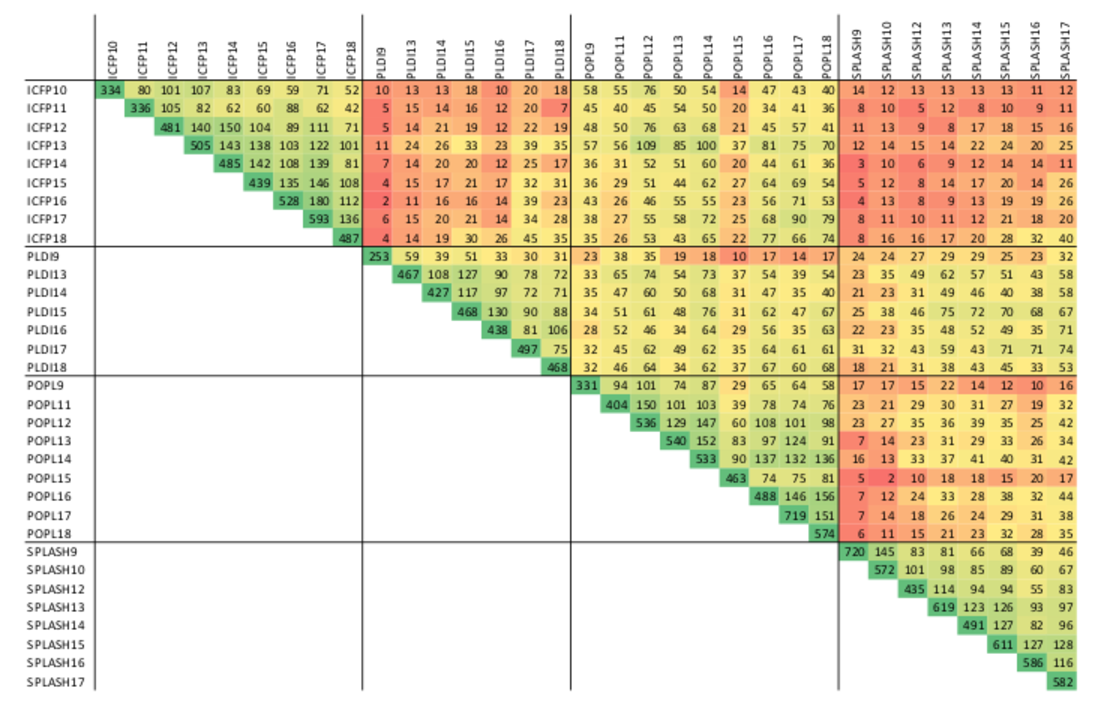
\includegraphics[width=\textwidth]{OverlapAnalysis-crop.pdf}
  \caption{Conference participation overlap.}
  \label{fig:overlap}
\end{figure}

Conversely, one can estimate the overlap for a given conference over time: for a
given conference at a time, and for any pair of years, compute the percentage of
attendees that participated in both events. This new information, as well as
the essential of Table~\ref{table:overlap-cross}, is synthesized graphically on
Figure~\ref{fig:overlap}.
With this bird-eye view of the permanence vs. transience of the
participants over time in SIGPLAN conferences, we can make a second observation,
temporal this time:

\begin{obs}
Temporal overlap is moderate: roughly a quarter of attendees at a given
conference were also present the year before at the same conference.
  \label{obs:overlap-temp}
\end{obs}

In principle, it is desirable to have a balance between repeat participants and
newcomers. Communities that don't attract new participants tend to stagnate; but
communities that don't have a core of repeat participants tend to lose focus.

The existence of a stable community associated with each conference series
(i.e., a group that
tends to repeat participation) is clearly visible near the diagonal in
Figure~\ref{fig:overlap}. The highest overlap of all in particular was between
ICFP'16 and ICFP'17, with 180 repeaters. The four conference series show
what seems to us to be a healthy balance between repeat participation and
newcomers.

The weaker overlap between conferences in different series is also apparent.
The strongest overlap is between PLDI and POPL, followed by ICFP and POPL
and by PLDI and SPLASH. The weakest overlaps are between ICFP and SPLASH,
followed by ICFP and PLDI, and by POPL and SPLASH. It is unclear whether the
overlap, or lack thereof, between these conference series is due to
intellectual reasons or due to their dates. PLDI and POPL is the pair that
is most distant in time, typically June and January. Conversely, ICFP and
SPLASH is the pair that is the closest in time, typically September and
October.  One might conjecture that temporal proximity discourages
cross-participation.

\begin{table}
  \centering
  \csvreader[%
    head to column names,
    tabular={|l|c|c|c|c|c|c|},
    table head=\hline \bfseries Conference & \bfseries Avrg & \bfseries Avrg $\geq$ 2 & \bfseries $\geq$ 2 (\%) & \bfseries $\geq$ 3 (\%) & \bfseries $\geq$ 4 (\%) & \bfseries $\geq$ 5 (\%) \\\hline,
    table foot= \hline,
    late after line=\ifthenelse{\equal{\Conference}{All}}{\\\hline}{\\},
  ]{../../output/sigplan/number_of_participations_per_conf.csv}{}{%
    \Conference & \csvcolii & \csvcoliii & \csvcoliv & \csvcolv & \csvcolvi & \csvcolvii
  }
\caption{For each conference and overall, the average number of instances a
  unique individual has taken part of (\textbf{Avrg}), and the same data without
  considering individual that has participated exactly once (\textbf{Avrg} $\geq$ \textbf{2}).
  The other columns display the percentage of participants that have
  attended at least $k$ instances, for $k\in\llbracket 2 \dots 5
  \rrbracket$. Note that the means and percentages are computed with
  respect to the number of \emph{unique} participants. }
\label{table:recurrent}
\end{table}

\begin{table}
  \centering
  \csvreader[%
    head to column names,
    tabular={|l|c|c|c|c|c|},
    table head=\hline \bfseries Year & \bfseries Avrg & \bfseries Avrg $\geq$ 2 & \bfseries $\geq$ 2 (\%) & \bfseries $\geq$ 3 (\%) & \bfseries $\geq$ 4 (\%) \\\hline,
    table foot= \hline,
    late after line=\ifthenelse{\equal{\Year}{All}}{\\\hline}{\\},
  ]{../../output/sigplan/number_of_participations_per_year.csv}{}{%
    \Year & \csvcolii & \csvcoliii & \csvcoliv & \csvcolv & \csvcolvi 
  }
  \caption{For each year, the average number of conferences a participant has participated
    in among POPL, PLDI, ICFP and SPLASH (\textbf{Avrg}),
    and the same data without considering individual that has participated exactly once (\textbf{Avrg} $\geq$ \textbf{2}).
  The other columns display the percentage of participants that have
  attended at least $k$ conferences, for $k\in\llbracket 2 \dots 4
  \rrbracket$. Note that the means and percentages are computed with
  respect to the number of \emph{unique} participants. }
\label{table:recurrent-year}
\end{table}


\begin{table}
  \centering
  \begin{subtable}[b]{0.4\textwidth}
    \centering
    \csvreader[%
      head to column names,
      tabular={|c|c|},
      table head=\hline \bfseries Year & \bfseries Old timers (\%)  \\\hline,
      table foot= \hline,
      late after line=\\,
    ]{../../output/sigplan/old_timer_POPL.csv}{}{%
      \year & \csvcolii 
    }
    \caption{Case of POPL}
  \end{subtable}
  \begin{subtable}[b]{0.4\textwidth}
    \centering
    \csvreader[%
      head to column names,
      tabular={|c|c|},
      table head=\hline \bfseries Year & \bfseries Old timers (\%)  \\\hline,
      table foot= \hline,
      late after line=\\,
    ]{../../output/sigplan/old_timer_ICFP.csv}{}{%
      \year & \csvcolii 
    }
    \caption{Case of ICFP}
  \end{subtable}
  \begin{subtable}[b]{0.4\textwidth}
    \centering
    \csvreader[%
      head to column names,
      tabular={|c|c|},
      table head=\hline \bfseries Year & \bfseries Old timers (\%)  \\\hline,
      table foot= \hline,
      late after line=\\,
    ]{../../output/sigplan/old_timer_PLDI.csv}{}{%
      \year & \csvcolii 
    }
    \caption{Case of PLDI}
  \end{subtable}
  \begin{subtable}[b]{0.4\textwidth}
    \centering
    \csvreader[%
      head to column names,
      tabular={|c|c|},
      table head=\hline \bfseries Year & \bfseries Old timers (\%)  \\\hline,
      table foot= \hline,
      late after line=\\,
    ]{../../output/sigplan/old_timer_SPLASH.csv}{}{%
      \year & \csvcolii 
    }
    \caption{Case of SPLASH}
  \end{subtable}
  \caption{For each conference, percentage of participants that have been
    part of a previous edition of the same conference.}
  \label{table:old-timers}
\end{table}

Finally, Table~\ref{table:recurrent} and \ref{table:old-timers} offer two
different views on recurrent participation. Table~\ref{table:recurrent}
represents respectively for the whole dataset (row ``ALL'') and for each
conference individually the average number of editions a participant has
been part of, as well as the percentage of participants that have been part
of at least a given number of editions of a conference. One striking fact is
that no less than 75\% of unique participants have been to just a single
edition.

Table~\ref{table:old-timers} is a normalization of the information represented
in Figure~\ref{fig:hist_attendance_per_conference}: for each instance of each
conference, it depicts the percentage of participants that have been part of a
previous instance of the conference (in our dataset). Since we take as origin of
time the first year for which we have data, the table is naturally overall monotonic
as years progress. Exceptions can be noticed, such as POPL'15, that seem to indicate
a (proportional) lack of ``old timers''. 

\begin{obs}
Over all conferences, the average number of conferences a given participant
has attended is just 1.52. Less than 4\% of unique participants have been to
more than five events among our dataset.  Similarly, at any given \event,
more than half of the participants were experiencing this conference for the
first time.
\label{obs:old-timers}
\end{obs}


\bcp{General question about all the pictures and tables: Are they
  consistent? (I.e., were the pictures generated from the data in the
  tables, or from earlier versions of that data?)}
\yz{Unfortunately no not at the moment: all tables are generated, but the
  Figures have been manually produced by Crista from her original take on
  the dataset. It would be great to regenerate them from the generated csv
  files, but I do not know how they have been generated exactly.}
